\documentclass[cover]{isas-seminar}

\usepackage{subfigure}
\usepackage{booktabs}
\usepackage{graphicx}
\usepackage{hyperref}

% Hier die Art der Veranstaltung eintragen (Seminar, Proseminar, Praktikum)
\eventtype{Praktikum} 
%\eventtype{Seminar} 
%\eventtype{Proseminar}
 
% Hier Titel der Veranstaltung eintragen 
\seminartitle{Forschungsprojekt Anthropomatik praktisch erfahren}
%\seminartitle{Modellbasierte Verfahren für intelligente Systeme}

\title{Projekt 2: Analyse von Schüttgutverhalten unter Verwendung von integrierter Sensorik}
\author{Andrea Bittner, Maren Kucza}

\begin{document}
\maketitle

\begin{abstract}
%Hier eine kommt die Zusammenfassung
%TODO Zusammenfassung
\end{abstract}
\clearpage
\tableofcontents
\cleardoublepage

\section{Einleitung}

Das Projekt basiert auf der FlexSort-Anlage, eine optische Bandsortieranlage für Schüttgut am Fraunhofer IOSB. Die Sortieranlage kann Schüttgut mit Hilfe einer Flächenkamera optisch klassifizieren und mittels Druckluftdüsen voneinander trennen. Damit eine konstante und gleich verteilte Menge von Schüttgut auf dem Band liegt, wird mittels Rüttler das Material freigegeben und rutscht über eine Rutsche auf das Band. Die nachfolgenden Abbildungen \ref{fig:k1_flexsort1} bis \ref{fig:k1_flexsort3} zeigen den FlexSort.

\begin{figure}[htb]
	\centering
	\begin{minipage}[t]{0.4\linewidth}
		\centering
		\includegraphics[width=1\linewidth]{images/k1-flexsort1.jpg}
		\caption{FlexSort: Schüttgut fällt vom oberen Querrüttler auf den kurzen Rüttler und rutscht dann auf das Sortierband}
		\label{fig:k1_flexsort1}
	\end{minipage}% <- sonst wird hier ein Leerzeichen eingefügt
	\hfill
	\begin{minipage}[t]{0.54\linewidth}
		\centering
		\includegraphics[width=\linewidth]{images/k1-flexsort2.jpg}
		\caption{FlexSort: Sortierband mit optischer Objekterkennung und Druckluftdüsen zum Ausblasen}
		\label{fig:k1_flexsort2}
	\end{minipage}
\end{figure}

\begin{figure}[htb]
	\centering
	\includegraphics[width=0.5\linewidth]{images/k1-flexsort3.jpg}
	\caption{FlexSort: Außenansicht mit großem Rüttler und Förderbändern um Schüttgut für geschlossenen Messlauf wieder nach oben zu befördern}
	\label{fig:k1_flexsort3}
\end{figure}
 
Da die Klassifizierung und das Ausblasen von Teilchen etwas verzögert stattfinden, ist eine zeitlich gut geplante Aktivierung der Druckluftdüsen notwendig, um die Anlage möglichst kostensparend und effizient zu betreiben. Hierfür muss die genaue Position der auszusortierenden Teilchen zum Zeitpunkt der Düsenüberquerung ermittelt werden. Dabei ist zu beachten, dass sich das Schüttgut vom Klassifizierungszeitpunkt bis zum Zeitpunkt des Ausblasens auf dem Band bewegt. Die Bewegung der Teilchen kann unter Umständen von einzelnen Parametern der Anlage beeinflusst werden und wirkt sich dadurch auf das Sortierergebnis aus. Beispielsweise kann die Geschwindigkeit des Bandes dazu führen, dass die Teilchen darauf springen oder der Rüttler durch ungünstige Vibrationsbewegungen keine konstante Menge von Teilchen über die Rutsche auf das Band frei gibt. 

In diesem Projekt soll eine Möglichkeit gefunden werden, den Prozess des Sortierens von Schüttgut genauer zu verstehen und dadurch weitere Optimierungen an der Anlage und im Prozess vornehmen zu können. So könnte ein stabileres Sortierergebnis erreicht werden. Neben den rein optisch gewonnen Daten können weitere Messwerte durch andere Verfahren unterstützend sein. In diesem Projekt soll dies mit Hilfe eines instrumentierten Schüttguts passieren, über den Bewegungsdaten gesammelt und ausgewertet werden können. Es soll untersucht werden, ob sich in den gewonnen Daten bestimmte Bewegungsmuster erkennen lassen, die auf einzelne Anlagenmodule zurückgeführt werden können. Gegebenenfalls lassen sich zwischen den Anlagenmodulen verschiedene Korrelationen erkennen, die zukünftig zur Optimierung der Anlage genutzt werden können. Darüber hinaus könnte ein Qualitätsmaß erstellt werden, anhand dessen die gewählten Parameter der Anlage bewertet werden.

 %Projektbeschreibung
\section{Projektplanung}

\subsection{Aufgabenstellung}

Im Rahmen des Forschungspraktikums soll ein Schüttgut konstruiert werden, dass über Sensorik verfügt, mit der genauere Positions- und Lagedaten gemessen werden können. Das Schüttgut soll die annähernde Größe des zu sortierenden Schüttguts haben. Die maximale Größe ist jedoch durch die Kapsel eines Überraschungs-Eis limitiert, in der die Sensorik untergebracht werden soll. Zunächst muss solch ein instrumentiertes Schüttgut entworfen werden.
 
Nach der Recherche von geeigneten Bauteilen soll ein Prototyp des Sensorik-Schüttguts erstellt werden, mit dem Daten auf einer Bandsortieranlage gewonnen werden können.

Zur Datengewinnung muss das Schüttgut programmiert werden, sodass die gelieferten Daten der Sensoren an eine Analysesoftware auf einem  PC/Laptop übertragen werden können. In einem weiteren Schritt sollen die gewonnen Daten ausgewertet werden. Hierfür muss eine Anwendung entwickelt werden, mit der sich die gewonnen Daten verständlich darstellen und analysieren lassen.
%TODO Qualtitätsmaß, Aufgabe anpassen
Die Werte der Sensoren müssen anschließend kalibriert und in Korrelation mit der tatsächlichen Laufbahn des Teilchens auf der Anlage gebracht werden. Hier soll eine Qualitätsgröße gefunden werden, die die Auswirkungen von verschiedenen Konfigurationsparametern der Anlage auf die Bewegung der Teilchen beschreibt und bewertet. 
Abschließend soll validiert werden, ob mit Hilfe von instrumentierten Schüttguts ein verbessertes Ergebnis der Bandsortieranlage erzielt werden kann.

Folgende Punkte beschreiben Herausforderungen, die großen Einfluss auf den weiteren Projektverlauf haben könnten:
\begin{description}
	\item [Begrenzte Größe:] Die Größe der Sensorik bestimmt zum einen, auf welche Anlage anschließende Messungen durchgeführt werden können, da das instrumentiertes Schüttgut zur Größenordnung des zu sortierenden Schüttgutes passen muss. Zum Anderen wirkt sich dies stark auf die Wahl der verwendeten Bauteile aus, die im verbundenen Zustand Platz in der Kapsel eines Ü-Eis finden müssen
	\item [Implementierung:] Gesammelte Daten über Sensoren müssen an den PC weitergeleitet werden. Hierfür gibt es verschiedene Möglichkeiten (Daten loggen oder per Funk direkt übertragen).
	\item [Bewertung der Daten:] Die gelieferten Daten von den Sensoren müssen aufbereitet werden, bevor sie interpretiert werden können.
	\item [Korrelation gemessene Daten zu Anlageparametern:] Finden einer Korrelation, Definition eines Qualitätsmaßes; Evaluation der Methode, durch instrumentiertes Schüttgut weitere Daten für die Optimierung der Anlage zu gewinnen 
\end{description} 

\subsection{Zeitliche Planung}
Die beschriebenen Herausforderungen spiegeln sich auch in den Meilensteinen des Projektes wieder:
\begin{description}
	\item [Meilenstein 1] beinhaltet das Design eines Schüttguts mit Sensorik, das die maximale Größe eines Ü-Eis hat. Zusätzlich wurde eine Machbarkeitsstudie durchgeführt, mit der die Wahl der Bauteile begründet werden kann.
	\item [Meilenstein 2] beinhaltet die Fertigung und Programmierung des Schüttguts mit Sensorik. Nach Abschluss liegt ein fertiges und funktionsfähiges instrumentiertes Schüttgut vor, das gemessene Daten per Bluetooth überträgt.
	\item [Meilenstein 3] umfasst das Sammeln und Darstellen von Daten aus der Anlage mit Hilfe des instrumentierten Schüttguts. Nach ausreichender Anzahl von Testdaten und Aufbereitung sowie Darstellung in einem Verständlichen Format ist der Meilenstein erreicht.
	\item [Meilenstein 4] beinhaltet die Analyse der Daten und die Findung einer Korrelation zu den Parametern der Schüttgutanlage. Eine gefundene Qualitätsgröße wurde definiert.
	\item [Meilenstein 5] schließt das Projekt mit der Evaluation der Ergebnisse ab. Es liegt nach Projektende eine Bewertung für das Verfahren vor, in dem mit  weiteren gewonnen Daten (außer den optischen) der Sortierprozess positiv beeinflusst werden kann.
\end{description}
	
Um das neue Verfahren zur Datengewinnung zu evaluieren, sind folgende Arbeitsschritte geplant: \newpage

\begin{figure}[ht]
	\centering
	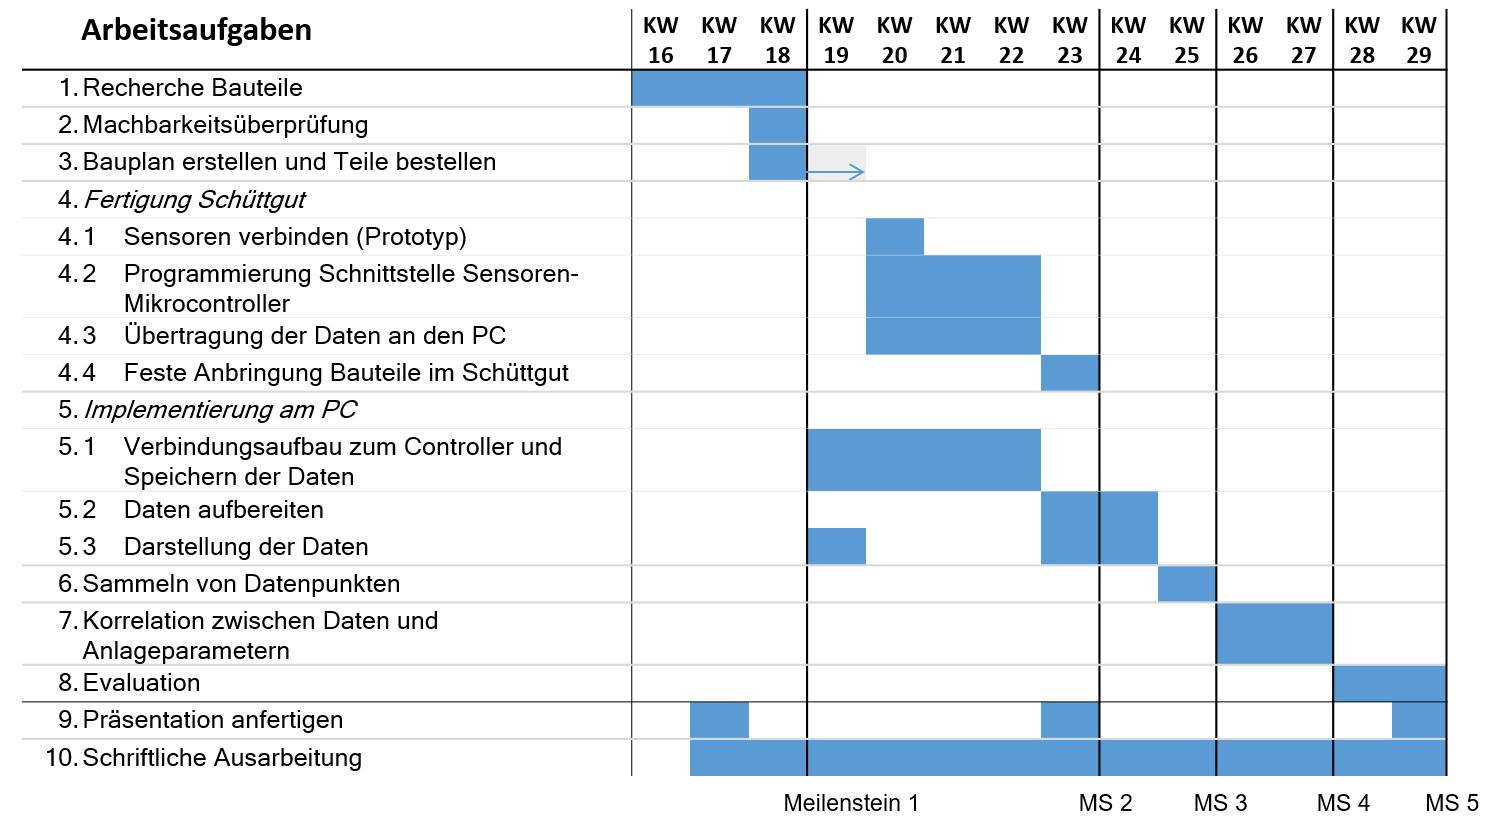
\includegraphics[width=1\textwidth]{images/k2-projektplan.JPG}
	\caption {Projektplanung runtergebrochen auf einzelne Arbeitsschritte}
	\label{fig:k2}
\end{figure}

Meilenstein 1 ist für die ersten drei Projektwochen angesetzt. Die grau markierte Kalenderwoche 19 bei Aufgabe 3 wird für die Bestelldauer der Bauteile geblockt. Solange kann nicht mit den Aufgabenteilen 4.* begonnen werden. Allerdings können einzelne Aufgaben aus Teil 5.* vorgezogen werden. Fortführend werden die Aufgaben 4 und 5 parallel bearbeitet, wobei Meilenstein 2 nach Kalenderwoche 23 ein fertiges instrumentiertes Schüttgut aufweist. Meilenstein 3 wird zwei Wochen später nach beenden von Aufgabenteil 5 und dem Sammeln von Testdaten erreicht. Ab Kalenderwoche 26 beginnt die Analyse der Daten für den Abschluss von Meilenstein 4. Die letzten beiden Wochen sind für die Evaluation des Projektes angesetzt, womit auch Meilenstein 5 erreicht wird. Zusätzlich sollte das Projekt fortlaufend dokumentiert sowie drei Präsentationen ausgearbeitet werden. %Projektplanung
\section{Arbeitsschritte}
 
\subsection{Design des instrumentierten Schüttguts}
\subsubsection{Kriterien für das instrumentierte Schüttgut}

Allgemeine Anforderungen an das instrumentierte Schüttgut:

\begin{itemize}
	\item Möglichst klein, maximale Größe der Module \textsuperscript{1\\)}
	\item Aufnehmen/Speichern von Bewegungsdaten
	\item Übertragung von Daten an einen PC
	\item Betrieben durch interne Batterie
	\item Optional: Cachen von Daten, bis diese ausgelesen werden 
\end{itemize}

\textsuperscript{1\\)} Das instrumentierte Schüttgut soll in eine Kapsel eines Kinder-Überraschungseis passen. Dadurch wird die maximale Größe des Schüttguts festgelegt. Die Wahl der Ü-Ei-Kapsel als Hülle für das Schüttgut eignet sich dahingehend gut, dass es einerseits den Mikrocontroller schützt, andererseits sehr einfach zu beschaffen ist und kein Behältnis aufwendig produziert werden muss (zum Beispiel mittels 3D-Druck).

\begin{figure}[ht]
	\centering
	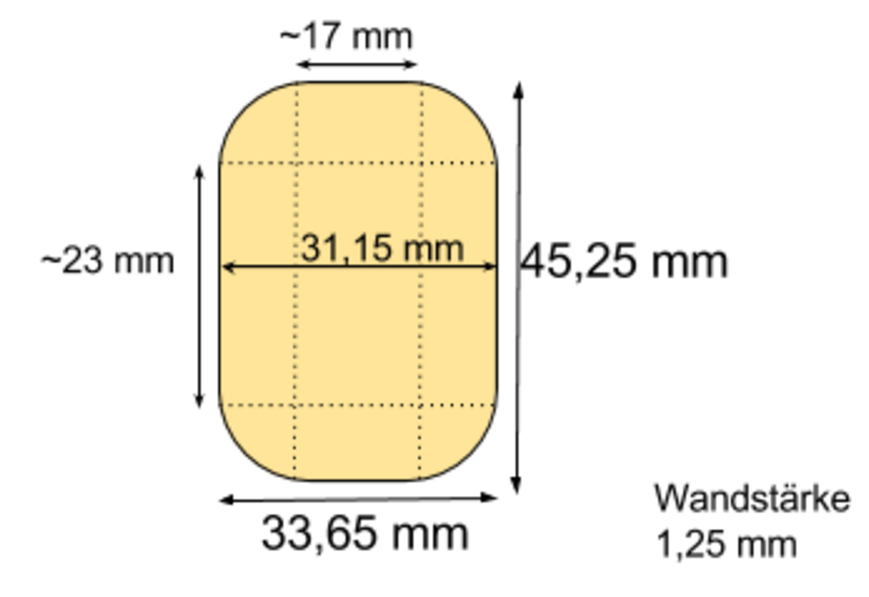
\includegraphics[width=0.5\textwidth]{images/k3-ueei.PNG}
	\caption {Maße der Kapsel aus einem Kinder Überraschungsei}
	\label{fig:k3}
\end{figure}

Die Beschaffung der Bauteile sollte zudem möglichst einfach sein. Von Vorteil ist, wenn alle Bauteile von einem deutschen Händler bezogen werden könnten, um einerseits nur einen einzelnen Liefervorgang zu haben und andrerseits eine geringere Lieferzeit (anstatt international). Auch eine ausreichende Dokumentation der einzelnen Module ist sehr nützlich für eine schnelle Implementierung des Mikrocontroller-Codes. Die einzelnen Module müssen kompatibel zueinander sein.

\subsubsection{Recherche}
Begonnen wurde mit einer Recherche, welche Bauteile es gibt, mit denen sich solch ein instrumentiertes Schüttgut erstellen lässt. Als Hauptplatine wird ein Mikrocontroller benötigt, an dem weitere Bauteile angeschlossen werden können. Es gibt einzelne Sensormodule, die z.B.Orientierung und Beschleunigung in je 3 Achsen gleichzeitig messen können. Ebenso gibt es verschiedene Speicher- und Übertragungsmodule, die Daten auf eine SD-Karte loggen oder per Bluetooth / WLAN / ZigBee weiterleiten können. Ausschlaggebend bei der Wahl der einzelnen Module war zunächst die Größe der einzelnen Bauteile, die selbst die Größe eines Ü-Eis nicht übersteigen dürfen. Nach der Wahl eines passenden Mikrocontrollers müssen auch die Anschlussmöglichkeiten für weitere Module mit beachtet werden.

\textbf{Mikrocontroller}, Gewähltes Bauteil: Adafruit Pro Trinket 3V 12MHz

Der Pro Trinket 3V 12MHz von Adafruit besitzt einen leistungsstarken ATmega328-Chip, der auch auf einigen Arduino-Mikrocontrollern verwendet werden. Er besitzt einen Speicher von 28K und einen RAM von 2K. Vorteile sind bei diesem, dass er jedoch mit 18 GPIOs (General Purpose Input Output) und 2 analogen Anschlüssen weitaus mehr Anschlussmöglichkeiten bietet, als beispielsweise der Arduino Pro Mini. Die Maße des Boards sind  38mm x 18mm x 4mm, sodass die Platine ausreichend Platz in der Kapsel haben sollte. Auf dem Trinket ist ein USB Bootloader vorinstalliert, sodass der Mikrocontroller per USB programmiert werden kann. (Quelle: \url{https://www.adafruit.com/products/2010}, 12.05.2016)

\textbf{Aufnahme von Bewegungsdaten}, Gewähltes Bauteil: Adafruit 9-DOF IMU Breakout - L3GD20H + LSM303

Das Modul L3GD20H kann drei verschiedene Datentypen in jeweils drei Achsen messen: Beschleunigungsdaten, Rotationsdaten und Magnetische Achsen ähnlich zu einem Kompass. Da Beschleunigungs- und Gyroskopdaten gemessen werden sollen, ist ein Bauteil, dass beide Daten zusammen liefern kann, sehr platzeffizient. Die Kommunikation zwischen dem Mikrocontroller und dem Datensensor benutzt das I2C-Protokoll. Das Bauteil hat die Maße 38mm x 23mm und ist damit um 5 Millimeter breiter als der Mikrocontroller Pro Trinket. (Quelle: \url{https://www.adafruit.com/products/1714}, 12.05.2016)

\textbf{Übertragung der Daten}

Zur möglichst unkomplizierten Übertragung von Daten an den PC wird eine drahtlose Verbindung verwendet. Dadurch ergeben sich drei verschiedene mögliche Typen:
\begin{itemize}
	\item ZigBee: Zu Aufwändig, da ein separates Modul für den PC benötigt wird. Hingegen sind fast alle Laptops heute standardmäßig mit WLan und Bluetooth ausgestattet.
	\item WLAN: Die zur Auswahl stehenden Platinen sind entweder deutlich zu groß, oder in ihrer Verwendung zu heikel, da sie extrem empfindlich auf kleinste Spannungsschwankungen reagieren. Zudem ist der Stromverbrauch größer als bei Bluetooth. Da das Schüttgut nur durch eine sehr kleine Batterie betrieben werden kann, ist dies hinderlich.
	\item Bluetooth: Bluetooth ist weit verbreitet und die Module sind klein genug, um sie mit im Ü-Ei unterzubringen.
\end{itemize}

Gewähltes Bauteil: Adafruit Bluefruit LE SPI Friend - Bluetooth Low Energy (BLE)

Gewählt wurde das Adafruit Bluefruit LE SPI Friend, dass durch Bluetooth Low Energy sehr energiearm sein soll. Zur Kommunikation mit dem Mikrocontroller wird das Protokoll SPI benutzt. Mit den Maßen 23mm x 26mm x 5mm ist es dicker als die anderen Bauteile, aufgrund der geringeren Breite sollte sich das Bauteil dennoch in der Rundung des Ü-Eis Platz finden. Das Modul hat außerdem Speicherplatz von 256KB. (Quelle: \url{https://www.adafruit.com/products/2633}, 12.05.2016)

\textbf{Betrieb durch interne Batterie}, Gewählte Bauteile: Adafruit Pro Trinket LiIon/LiPoly Backpack Add-On, Lithium Ion Polymer Battery - 3.7v 150mAh

Um einen universellen Einsatz des instrumentierten Schüttguts zu garantieren, muss es mit einer eigenen Batterie oder einem eigenen Akkumulator betrieben werden. 
Mit dem Adafruit Trinket Lilon Backpack Add-On lässt sich ein Akkumulator an das Pro Trinket anschließen. Das Add-On dient als Ladestation, wenn das Pro Trinket per USB mit einem Rechner verbunden ist. Sobald der USB-Port entfernt wird, schaltet das Modul automatisch in den batteriebetriebenen Modus. Das Modul hat eine Größe von 15mm x 17mm x 7mm. Die relativ große Höhe im Vergleich zu den anderen Modulen kommt durch den Anschluss für den Akkumulator zustande. (Quelle: \url{https://www.adafruit.com/products/2124}, 12.05.2016)

Hinzu kommt eine Lithium Ion Polymer Battery mit 3,7V und 150mAh. Dieser Akku wurde aufgrund der geringen Größe von 19,75mm x 26mm x 3,8mm gewählt. Es gibt auch Modelle mit mehr Kapazität, die aber auch andere Abmessungen besitzen. Zum Teil geht die Länge über 30mm hinaus. Es werden allerdings schon Bauteile über diese Länge verwendet, die in der vertikalen Achse der Kapsel platziert werden müssen. Der Akku sollte daher näher an der Aussenwand positioniert werden, wo die Höhe durch die Abrundung der Kapsel jedoch eingeschränkt wird. (Quelle: \url{https://www.adafruit.com/products/1317}, 12.05.2016)

\textbf{Alternative Überlegungen zum Cachen der Daten}

Da die meisten Mikrocontroller nur sehr wenig eigenen Speicher haben und eine drahtlose Datenverbindung nicht zuverlässig genug ist, müssen die vom Sensor gelesenen Daten auf einem extra hinzugefügten Speicher zwischen gespeichert werden, bis sie vom PC ausgelesen werden können.

Mögliche Bauteile: Adafruit I2C Non-Volatile FRAM Breakout - 256Kbit / 32KByte (Quelle: \url{https://www.adafruit.com/products/1895}, 12.05.2016), Adafruit SPI Non-Volatile FRAM Breakout - 64Kbit / 8KByte (Quelle: \url{https://www.adafruit.com/products/1897}, 12.05.2016) 

Vorerst sind diese Bauteile out of scope, da das Bluetooth Modul über 256 KB Speicher verfügt, die eventuell als Cache bzw. Puffer genutzt werden können.
Mit den gewählten Bauteilen lässt sich der Speicher des Mikrocontrollers von den integrierten 28 KB (schon abzüglich der 4 KB für die Dateien des Bootloaders) auf um 8 bzw. 32  KB erhöhen. 

Die gewählten Bauteile sind alle von der Marke Adafruit. Der Vorteil darin liegt in der Kompatibilität der Bauteile aufgrund der Abstimmung zueinander, sowie in der sehr ausführlichen Dokumentation dieser. 

\textbf{Verwendete Hardware}

\begin{table}[h]
	\centering
	\begin{tabular}{|l|c|}
		\hline
		\textbf{Bauteil} & \textbf{Menge} \\
		\hline
		 Adafruit Pro Trinket 3V 12MHz & 3 \\
		 \hline
		 Adafruit 9-DOF IMU Breakout - L3GD20H + LSM303 & 3 \\
		 \hline
		 Adafruit Bluefruit LE SPI Friend - Bluetooth Low Energy (BLE) & 3 \\
		 \hline
		 Adafruit Pro Trinket LiIon/LiPoly Backpack Add-On & 3 \\
		 \hline
		 Lithium Ion Polymer Battery - 3.7v 100mAh\textsuperscript{*)} & 9 \\
		 \hline		 
	\end{tabular}
		\caption{Bestellte Hardware}
		\label{tab:bestellteHW}
\end{table}

\textsuperscript{*)} Aufgrund von der Nichtverfügbarkeit des gewünschten Akkus bei einem Lieferanten musste ein anderer Akku gewählt werden. Dadurch konnte die Bestellung aber bei nur einem Lieferanten getätigt und eine kurze Lieferzeit erreicht werden.

\begin{table}[h]
	\centering
	\begin{tabular}{|l|c|}
		\hline
		\textbf{Materialien} & \textbf{Menge} \\
		\hline
		Breadboard & 2 \\
		\hline
		Set mit Steckkabeln & 2 \\
		\hline
		Arduino Uno & 1 \\
		\hline	
		Arduino Duemilanove & 1 \\
		\hline	
		Ardunio Feather & 1\\
		\hline
	\end{tabular}
	\caption{Weitere Hilfsmittel stehen zur Verfügung}
	\label{tab:verfuegbareHW}
\end{table}

\subsubsection{Machbarkeitsstudie}

Vor der Bestellung wurden noch einige Machbarkeitsstudien durchgeführt. Neben dem Vergleich gegenüber anderen verfügbaren Modulen wurde ein Größentest durchgeführt und eine Wiring-Skizze angefertigt.

Bei dem Größentest wurden die einzelnen Module Maßstabsgetreu mit Moosgummi nachgebaut. Dadurch konnte getestet werden, wie sich die Module am besten in der Ü-Ei-Kapsel anordnen lassen. Zusätzlich sollte in der Kapsel aber noch genügend Freiraum sein, da auch die einzelnen Kabelverbindungen zwischen den Modulen Platz benötigen.  \\
Wie in Abbildung \ref{fig:k3_machbarkeitsstudie} ersichtlich wird, passen alle Module in die Kapsel und es ist noch ausreichend Platz für Verbindungen.

\begin{figure}[ht]
	\centering
	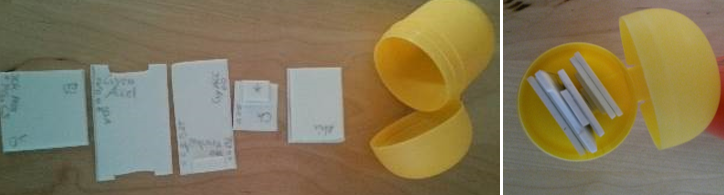
\includegraphics[width=1\textwidth]{images/k3-machbarkeitsstudie.PNG}
	\caption {Machbarkeitsstudie: Nachbau der Module mit Hilfe von Moosgummi}
	\label{fig:k3_machbarkeitsstudie}
\end{figure}

Die Wiring-Skizze in Abbildung \ref{fig:k3_wiringskizze} zeigt die Verbindungen der einzelnen Module untereinander. Diese ist nicht maßstabsgetreu. Ziel war es, alle Module korrekt miteinander verbinden zu können. Damit konnten auch schon erste Überlegungen angestellt werden, wie die Module später auch in der Kapsel angeordnet werden könnten. Letztendlich wird die Skizze auch hilfreich beim Löten sein.

\begin{figure}[h]
	\centering
	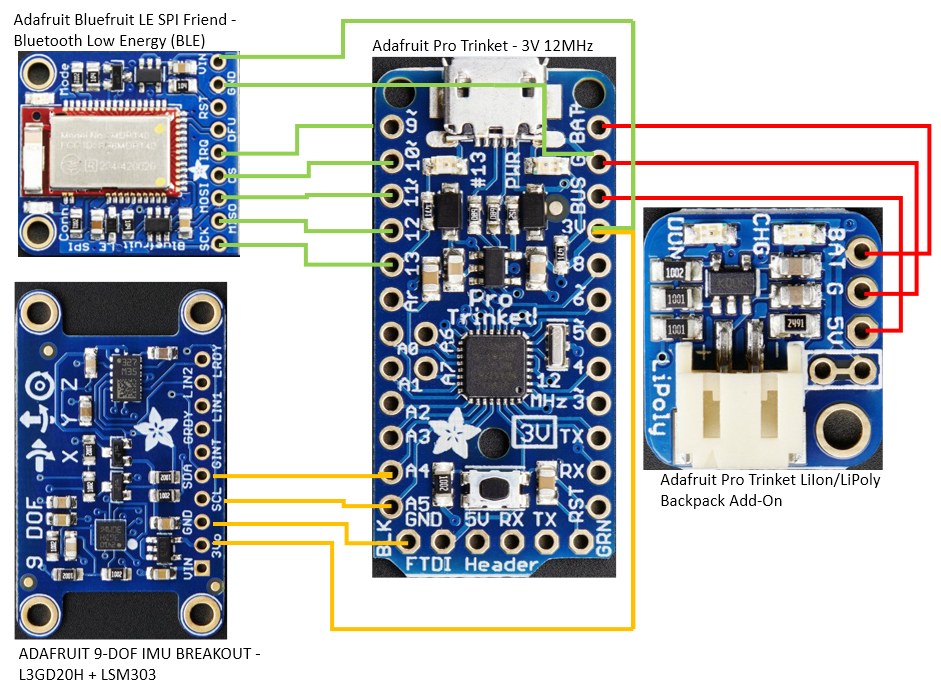
\includegraphics[width=0.9\textwidth]{images/k3-wiringskizze.PNG}
	\caption {Wiring-Skizze, wie die Bauteile miteinander verbunden werden}
	\label{fig:k3_wiringskizze}
\end{figure}

Nach positiven Ergebnissen aus den Machbarkeitsstudien wurden die Bauteile wie sie in Tabelle \ref{tab:bestellteHW} aufgeführt sind, bestellt. Da die Bestellung bei einem Händler getätigt wurde, waren die Bauteile in der folgenden Woche schon verfügbar.
\newpage

\subsubsection{Prototyping}

Für einen ersten Prototyp wurden die Bauteile mit Hilfe eines Breadboards und Steckkabeln miteinander verbunden. Zuerst wurden die Pro Trinkets getestet. (Hier ist leider ein Defekt eines Pro Trinkets aufgefallen.) Anschließend wurde das Bluetooth-Modul und zum Schluss das Sensor-Modul hinzugenommen.

\begin{figure}[h]
	\centering
	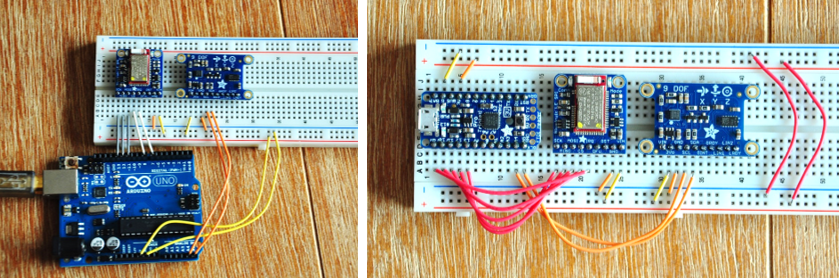
\includegraphics[width=1\textwidth]{images/k3-prototyping.PNG}
	\caption {Links: Prototyping mit dem Arduino Uno; Rechts: Prototyping mit dem Adafruit Pro
		Trinket}
	\label{fig:k3_prototyping}
\end{figure}

An dieser Stelle wurde außer dem Adafruit Pro Trinket noch ein Arduino Uno hinzugenommen, um während der Programmierung des Mikrocontrollers (siehe Kapitel \ref{kapitel_programmierungMikrocontroller}) auch mit einer Seriellen Ausgabe testen zu können. Bei erfolgreichem Testen des Programmcodes wurde dieser dann auf den Adafruit Pro Trinket übertragen.
%Erwähnen warum Uno schon vorher?

\subsubsection{Löten}

Da drei Bausätze vorhanden waren, und nur einer für das Prototyping genutzt wurde, konnte mit dem Löten des ersten Bausatzes begonnen werden, der in die Ü-Ei Kapsel passen soll.
Abbildung \ref{fig:k3_erstesBauteilGeloetet} zeigt das fertig gelötete Bauteil.

\begin{figure}[ht]
	\centering
	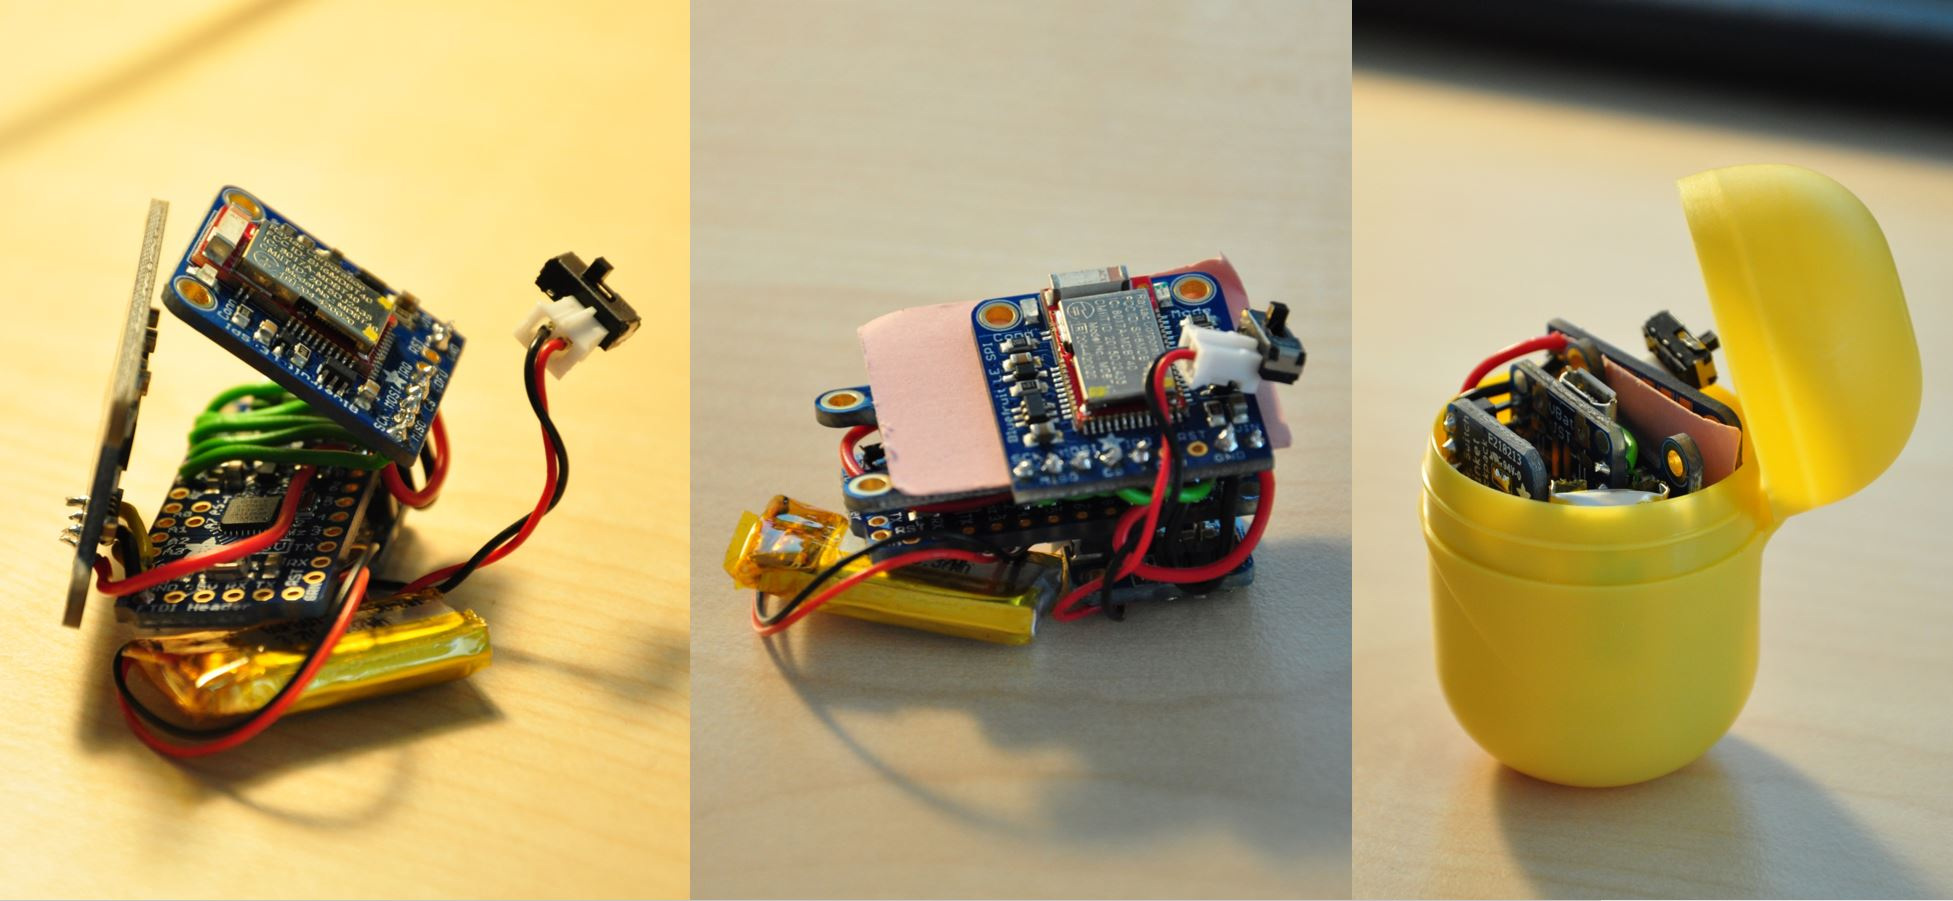
\includegraphics[width=1\textwidth]{images/k3-erstesBauteilGeloetet.jpg}
	\caption {Links: das erste gelötete Bauteil; Mitte: zwischen dem Bluetooth- und dem Sensor-
		Modul wird Papier zur Isolierung verwendet; Rechts: das Bauteil passt in eine Ü-Ei-Kapsel}
	\label{fig:k3_erstesBauteilGeloetet}
\end{figure} %Projektdurchführung
\subsection{Programmierung des Mikrocontrollers}
\label{kapitel_programmierungMikrocontroller}
 
\subsubsection{Benötigte Software}

Zur Programmierung des Mikrocontrollers musste zunächst notwendige Software und Treiber geladen und installiert werden.

\begin{description}
	\item[Entwicklungsumgebung] Arduino IDE (1.6.8), für die Programmierung des Arduino Chip ATmega328, der auf dem Adafruit Pro Trinket verbaut ist
	\item[Bootloader] Innerhalb der Arduino IDE muss der Bootloader Adafruit AVR Boards (1.4.7) installiert werden
	\item[Treiber für die Adafruit Module] Adafruit\_driver, Adafruit\_9DOF, \\ Adafruit\_BluefruitLE\_nRF51, Adafruit\_Sensor, Adafruit\_LSM303LHC, \\ Adafruit\_L3GD20\_U, Adafruit\_BMP085\_Unified
\end{description}

Adafruit stellt außerdem über Google Play die Android-App ,,Adafruit Bluefruit LE Connect'' zur Verfügung, über die mit Hilfe der beigefügten Testbeispiele in den Treiberpacketen das Bauteil mit dem Smartphone verbunden und ausprobiert werden kann. 

Für das Projekt wurde eine eigene Android-App entwickelt, die in Kapitel \ref{AndroidAppFürDatenmessen} beschrieben wird.

\subsubsection{Programmieren des Mikrocontrollers}
% setup, loop()
Da der Adafruit Pro Trinket keinen seriellen Ausgabeport hat, wurde die Programmierung zuerst auf einen Arduino Uno geladen, der wie auf der linken Seite der Abbildung \ref{fig:k3_prototyping} mittels eines Breadboards mit den Adafruit-Modulen war. Während der Programmierung konnte mittels \texttt{Serial.print()}-Befehlen der Programmablauf auf dem Mikrocontroller kontrolliert werden, bis er anschließend auf den Adafruit Pro Trinket übertragen werden konnte.

Das finale Programm besteht aus zwei Dateien. Nach dem ersten Testlauf wurden die App nochmals überarbeitet und auch die Android-App zum Datenempfang dazu angepasst. Die Datei \texttt{BluefruitConfig.h} beinhaltet die Festlegungen der verwendeten Pinouts des Mikrocontrollers zur Funktion. Der eigentliche Programmcode befinden sich in der \texttt{Program.ino}, die im nachfolgenden grob erklärt wird.

Zunächst werden Bibliotheken für die Adafruit Module eingebunden, sowie eine Instanz erstellt, die eine Bluetooth Low Energy-Verbindung aufbaut. Nun gibt es eine \texttt{Setup()}-Funktion, die nur einmal beim Start des Mikrocontrollers aufgerufen wird. Hier wird eine Bluetooth-Verbindung aufgebaut und die Sensoren initialisiert. Danach folgt die \texttt{Loop()}-Funktion, die wiederholt aufgerufen wird. Da diese auch auf gesendete Befehle der Android-App reagiert, wird die Funktion mittels Struktogramm in Abbildung \ref{fig:k3_loopstructo} erklärt.

\begin{figure}[h]
	\centering
	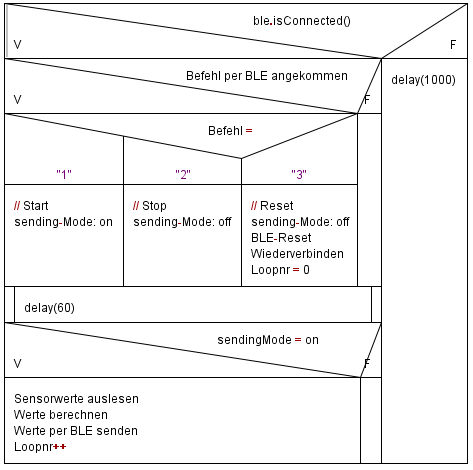
\includegraphics[width=0.9\textwidth]{images/k3-loopstructo.png}
	\caption {Struktogramm des Codeinhaltes der \texttt{loop()}-Methode}
	\label{fig:k3_loopstructo}
\end{figure}

Besteht keine BLE-Verbindung, wartet der Mikrocontroller 1000ms, bis er wieder mit dem erneuten Aufruf von \texttt{loop()} beginnt. Bei bestehender Verbindung wird zunächst eventuelle empfangene Befehle der Android-App ausgewertet. Sollen Daten gesendet werden (\texttt{Senden-Modus = on}), wird mit dem Auslesen der Sensor-Werte und dem Sende dieser per BLE fortgefahren. 


\subsection{Empfangen der Messwerte}

\subsubsection{BLE Clients mit Python}
Für den Client wurde Python verwendet, da es zum einen leicht zu verwenden ist, zum anderen von Adafruit eine Bibliothek zum Verbindungsaufbau mit einem BLE Modul bereitgestellt wird. Durch die beigefügten Beispiele wäre der Verbindungsaufbau mit dem Laptop sehr einfach gewesen und eine Echtzeitdarstellung der ankommenden Daten möglich. Unklar war jedoch, dass es in dem benötigten Modul 'dbus' zu einem Attributeerror kommt. Da dieser nicht gelöst werden konnte, wurde eine Alternative entwickelt.

\subsubsection{Alternativ Client zum Empfang der Daten per BLE: Android App}
\label{AndroidAppFürDatenmessen}
Da es bereits die Android-App ,,Adafruit Bluefruit LE Connect'' gibt, mit der Daten per BLE empfangen und gesendet werden können, konnte davon ausgegangen werden, dass in der Konstellation Smartphone-Bluefruit-Modul BLE-Verbindungen funktionieren und unterstützt werden. Daraus ergibt sich auch der Vorteil, dass ein Smartphone als Empfänger wesentlich mobiler ist, um an der Anlage am Sender mitlaufen zu können. 

Von Adafruit gibt es über Github\footnote{Github-Link: \url{https://github.com/adafruit/Adafruit_Android_BLE_UART}} die Klasse ,,Adafruit Android BLE UART'', mit der eine BLE-Verbindung zu einem Bluefruit-Modul von einem Android-Smartphone aus hergestellt werden kann. Dabei handelt es sich um eine abgespeckte Variante der App oben erwähnten App. Mit Hilfe des Codes für BLE-UART-Verbindungen wurde eine App entwickelt. Als Entwicklungsumgebung kam Android Studio zum Einsatz. Neben dem BLE-Aufbau muss die App Befehle an den Mikrocontroller senden können. Sobald Sensordaten vom Mikrocontroller ankommen, sollen diese Werte in lokalen Dateien gespeichert werden.

Zuerst musste eine Verbindung mit dem Bluefruit-Modul hergestellt werden. Bei eingeschaltetem Bluetooth am Smartphone sucht die App automatisch nach BLE-Geräten. 

Die App verfügt über vier Buttons, um das Verhalten des Mikrocontrollers sowie das Speichern der Daten kontrollieren zu können:
\begin{description}
	\item[Start] Sendet einen Start-Befehl an den Mikrocontroller, damit dieser mit dem Senden von gemessenen Sensordaten beginnt
	\item[Stop] Sendet einen Stop-Befehl an den Mikrocontroller, damit dieser mit dem Senden von gemessenen Sensordaten stoppt. Die gemessenen Daten bleiben dabei in einem String Buffer vorhanden
	\item[Save] Speichert die gemessenen Daten in einem neuen File ab. Dabei werden genutzte Zähler nicht zurückgesetzt. Der Button kann benutzt werden, um bei einem Messlauf markante Punkte auf der Anlage zu markieren, indem ein neues File erstellt wird. Zusätzlich wird die Performanz verbessert.
	\item[Reset \& Save] Speichert die gemessenen Werte in ein File und setzt anschließen genutzte Zähler zurück. Zusätzlich wird ein Reset-Befehl an den Mikrocontroller gesendet, um die BLE-Verbindung neuzustarten und ebenfalls Zähler zurückzusetzen. Bei erfolgreicher Wiederverbindung, beginnt direkt wieder der Datenempfang, sofern der Mikrocontroller vorher auch im Senden-Modus war. Der Button kann benutzt werden, um bei einem Messlauf eine neue Runde auf der Anlage zu markieren, sowie eine gute Performanz zu behalten, indem gespeicherte Felder nicht zu groß werden.
\end{description}

\begin{figure}[h]
	\centering
	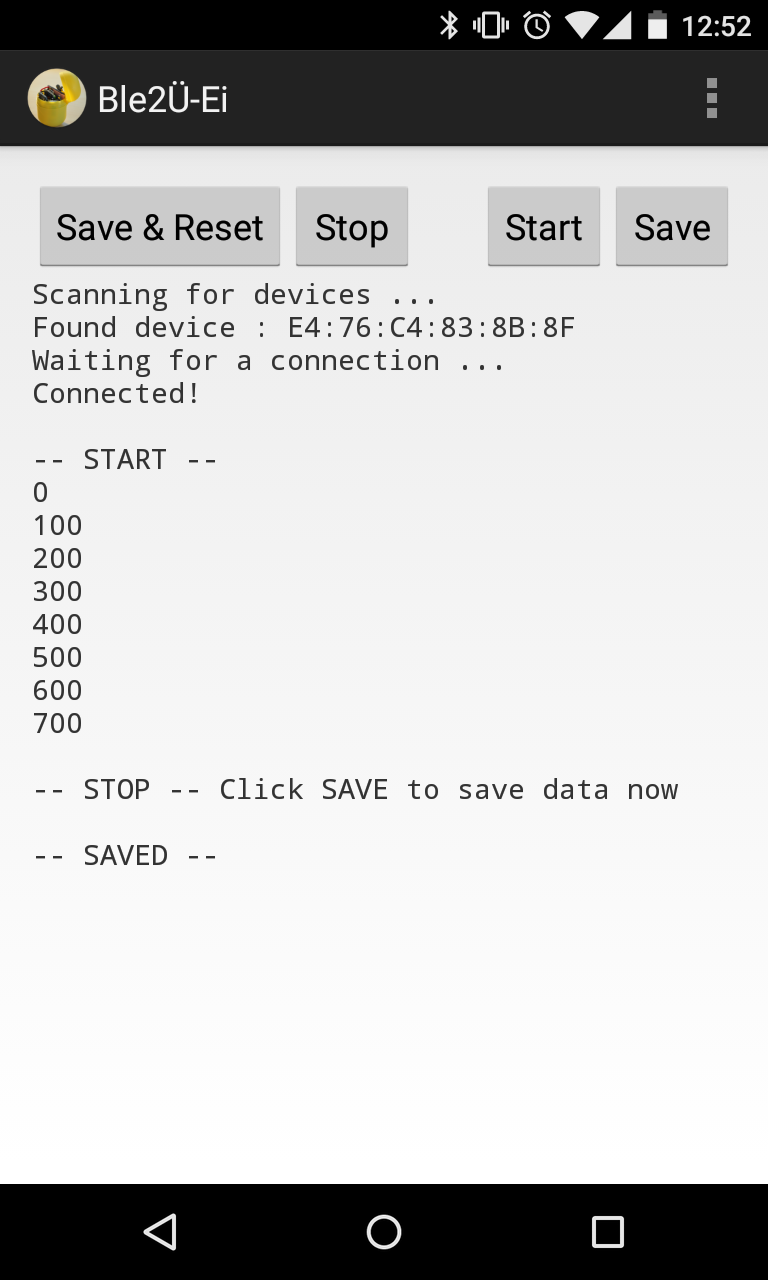
\includegraphics[width=0.45\textwidth]{images/k3-androidapp.png}
	\caption {Android-App zum Steuern des Mikrocontrollers und Empfangen der Sensordaten}
	\label{fig:k3_androidapp}
\end{figure}

Die Daten werden in Dateien lokal auf dem Smartphone gespeichert und müssen anschließend auf einen Rechner übertragen werden. Derzeit ist der ,,Download''-Ordner des Smartphones fest implementiert. Hier gibt es sicher noch Potential zur Erweiterung, indem die Daten direkt über einen Data Service an einen PC oder Laptop weitergeleitet werden könnten oder zumindest der Speicherort variabler wird. \\
Abgelegt werden die Files in einem bestimmten Namensformat. Sie beginnen mit dem aktuellen Timestamp um identische Filenamen zu verhinden. Zusätzlich wird noch der Bereich mittels eines internen App-Zählers angegeben, um zusammenhängende Dateien für eine Messrunde identifizieren zu können.
\subsection{Client zur Datenanalyse}

Der Client ist in Python implementiert, da zum Zeitpunkt, als die Probleme in der Adafruit BLE Library bekannt wurden, bereits große Teile des Clients implementiert waren. Zudem ist Python sehr leicht erlernbar und bietet gute Bibliotheken für eine Vielfalt von Anwendungsfällen.
\subsubsection{Graphisches User Interface}
Für die Darstellung graphischer Bedienelemente im Client, wurde die Library \texttt{PyQt4} verwendet, die eine leichte Integration der Graphen der Sensordaten ermöglicht. Diese werden mit Hilfe einer anderen Bibliothek erzeugt, können aber als ein sogenanntes Widget leicht in die GUI integriert werden.
Da keine Echtzeitübertragung der Daten möglich ist, werden nur wenige Bedienelemente, welche in einer Menuleiste untergebracht sind, benötigt:
\begin{itemize}
\item Öffnen einer Testdatei
\item Anzeigen von Statistiken über den Testlauf (Dauer des Testlaufs, gemessene minimal und maximal Werte)
\item Zusammenfügen von Dateien, wenn ein Testlauf in verschiedenen Dateien gespeichert ist
\item Parametrisieren und Anwenden des Filters
\end{itemize}
Werden vom Nutzer ungültige Eingaben gemacht, wird ihm dieser Fehler durch Dialogfenster mitgeteilt. 
\subsubsection{Datenformat}
Um alle weiteren Verarbeitungsschritte zu erleichtern wird ein einfaches Datenformat, welches Json ähnelt, verwendet. Die ausgelesenen Sensordaten werden in einem Tupel zusammen mit einem Zeitstempel, einer fortlaufenden Nummer und einer ID, welches den verwendenten Mikrocontroller identifiziert, gesendet.
\begin{figure}[h]
	\centering
	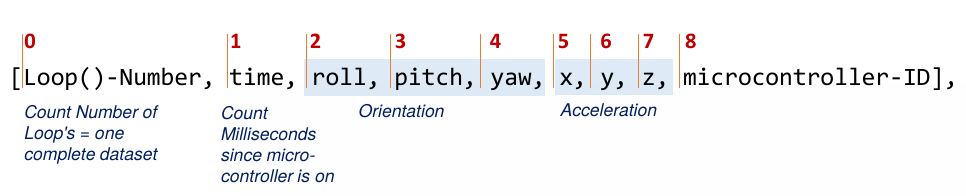
\includegraphics[width=1\textwidth]{images/k3-datenformat.png}
	\caption {Eingesetztes Datenformat}
	\label{fig:k3-datenformat.png} 
\end{figure}
\subsubsection{Parser}
Der Parser operiert auf oben beschriebenen Datenformat und hat zwei Hauptaufgaben:
\begin{itemize}
 \item Bereinigen der Daten, falls unvollständige, oder inkorrekte Tupel ankommen
 \item Aufteilen der Daten in Arrays, welche dann als Graph dargestellt werden können
\end{itemize}
Durch Eingabe einer Datendatei werden sechs Listen erzeugt, welche zur Darstellung and die Klasse \texttt{Plotter} übergeben werden. Die ersten drei Listen enthalten die Daten der drei Gyroskop Achsen, die letzen drei Listen die Daten der Achsen des Beschleunigungssensors. Da für die Werte der x-Achse die Zeitstempel verwendet werden, enthalten diese Listen jeweils Tupel der Form \texttt{(Zeitstempel, gemessener Wert)}.
\subsubsection{Darstellen von Daten}
Das Erzeugen der Graphen erfolgt in der Klasse \texttt{Plotter}, welche die Bibliotheken \texttt{numpy} und \texttt{pyqtgraph} verwendet. Für den Filter wird zudem noch die Bibliothek \texttt{scipy} benötigt. Durch \texttt{pyqtgraph} wird ein \texttt{PlotWidget} erzeugt, welches genau einen Graphen beinhaltet, der entweder die Werte der drei Achsen des Gyroskops oder des Beschleunigungssensors darstellt. Die y-Achse ist in der Einheit $\dfrac{\circ}{s}$ bei ersterem Graph und $\dfrac{m}{s^{2}}$ bei letzterem. Die x-Achse ist in beiden Graphen der Zeitstempel des Datentupels. (In \ref{fig:k3_4-graph.png} ist ein solcher Graph beispielhaft dargestellt).
\begin{figure}[h]
	\centering
	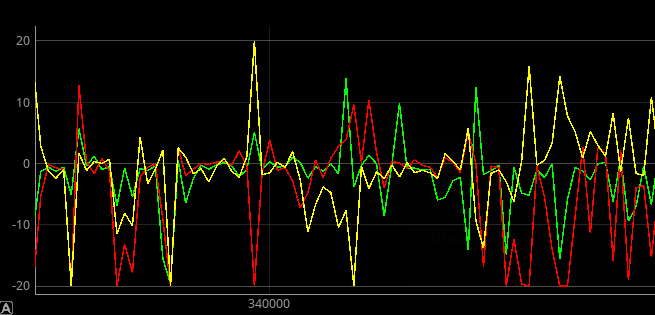
\includegraphics[width=0.75\textwidth]{images/k3-graph.png}
	\caption {Beispielgraph}
	\label{fig:k3_4-graph.png} 
\end{figure}
Ein \texttt{PlotWidget} enthält ein \texttt{PlotItem} welches eine Menge von \texttt{PlotDataItems} enthält, d.h. eine Menge von gemessenen Datenpunkten.
Für jeden der beiden Graphen wird dann in der Klasse \texttt{Presenter} eine Instanz der Klasse \texttt{Plotter} erzeugt und zu einer \texttt{QVBoxLayout} hinzugefügt. Diese dient dazu, die einzelnen enthaltenen Widgets relativ zueinander anzuordnen.
Damit die Graphen unabhängig der Anzahl der enthaltenen Datenpunkte gleichgroß dargestellt werden, wird die Größe des Fensters für jeden Graphen neu berechnet. Übersteigt die Größe des Graphen die Größe des Fensters, wird automatisch die horizontale Scrollbar angepasst.
\subsubsection{Datenaufbereitung}
Durch verschiedene äußere Bedingungen (z.B. Empfindlichkeit des Sensors oder Vibration der Bahn) werden die gemessenen Rohdaten verfälscht. Durch Anwendung von Filtern, können die Daten verbessert werden.
Hierbei wurden zwei Ansätze betrachtet, aber nur einer implementiert:
\begin{enumerate}
\item Savitzky-Golay-Filter
\item Kalman-Filter
\end{enumerate}
\paragraph{Savitzky-Golay-Filter}
Das Savitzky-Golay-Filter ist ein einfaches Glättungsfilter, bei dem auf die Daten der Kurve innerhalb eines Fensters eine polynomiale Regression angewandt wird. Das Filter hat gute Eigenschaften, wenn es um die relative Verteilung von Maxima und Minima geht. Es ist wahrscheinlich, dass durch die Empfindlichkeit der Sensoren bereits kleinste Vibrationen der Bahn aufgezeichnet werden. Diese geben jedoch kaum Aufschluss, in welchem Abschnitt der Sortieranlage sich das Schüttgut derzeit befindet. Größere Bewegungen, die auch in größeren Ausschlägen in den Sensoren resultiern, sind dafür besser geeignet. Insofern ist der Erhalt der Maxima und Minima von Nutzen.
Die Parameter, die bei diesem Filter verändert werden können, sind die Fensterbreite und der Grad des Polynoms. Je größer das Fenster und desto niedriger der Grad, desto mehr wird die Kurve effektiv gedämpft.
\paragraph{Kalman-Filter}
Das Kalman-Filter zieht im Gegensatz zum Savitzky-Golay-Filter zwei verschiedene Arten von Rauschen in betracht:
\begin{itemize}
\item Prozessrauschen 
\item Sensorrauschen
\end{itemize}
Jedoch ist die Wahl und Beschreibung des zu Grunde liegenden Systems entscheidend für die Parameterwahl. Ist das System nur unzureichend bekannt und wird deshalb schlecht beschrieben, ist der Filter nicht mehr als ein Tiefpass und wird keine guten Ergebnisse liefern. Da in unserem Fall die Erfahrung in der Anwendung eines solchen Filters fehlt, wurde dieser Ansatz bereits nach kurzer Zeit verworfen.
Die Wahl der Parameter ist beim Einsatz von Filtern entscheidend. Diese haben großen Einfluss auf die Form des resultierenden Graphen. Das macht sie aber auch besonders problematisch, da sie meist nur experimentell ermittelt werden können und unklar bleibt, wie weit die Graphen tatsächlich geglättet werden müssen, um ein verwertbares Ergebnis zu erhalten. 
\section{Datenmessung}

\subsection{Erkenntnisse aus dem ersten Testlauf}
Nach dem ersten Testlauf mit der Android-App und dem Bauteil konnten neue wichtige Erkenntnisse gewonnen werden.
Zwischen der App und dem Mikrocontroller kam es zu häufigen Verbindungsabbrüchen. In der App gibt es noch einige Unstimmigkeiten, die behoben werden sollten, damit verwertbare Daten aufgezeichnet werden können. 

\begin{itemize}
	\item Es muss einen fortlaufenden Zähler vom Mikrocontroller aus geben, damit nach einem Verbindungsabbruch und -wiederaufbau der Zähler mitten im Durchlauf nicht auch wieder bei 0 beginnt
	\item Beheben eines Bugs im beim Datenaufzeichnen nach dem ersten Verbindungsabbruch
	\item Der Zugriff auf die UI-Elemente ist zu hoch. Die Ausgabe auf die UI ist langsamer, als die eingehenden Daten, weshalb die App ab vielen Ausgaben eingefrohren ist. Ab dann konnten bisher empfangene Daten auch nicht mehr gespeichert werden
	\item Das Speichern sollte performanter sein
	\item Wie lässt sich ein Rundendurchlauf bzw einzelne markante Punkte in der Anlage währen der Datenaufzeichnung markieren, um nachträglich die analysierten Daten evaluieren zu lassen?
	\item Bluetooth funktioniert über eine Reichweite zwischen 5-10 Metern. Bei zu vielen Verbindungsabbrüchen muss mit dem Empfangsgeräte an der Anlage mitgelaufen werden, da die Wände der Anlage etwas zu abschirmend sind. Eventuell gibt es eine Möglichkeit mehrere BLE-Empfänger an der Anlage zu positionieren
	\item Zum Schutz des Bauteils wurde die Kapsel in Polsterfolie eingepackt. Dadurch wurde das Bauteil langsamer durch die Anlage befördert als die Steine
	\item Ein Akku mit 100 mAh hält doch länger als anfangs angenommen
\end{itemize}

\subsection{Hauptlauf}

Nach Optimierung der Android App konnten wieder Daten gemessen werden. Die Bluetooth-Verbindungsaufbau wurde verändert, sodass die Verbindung nun viel stabiler lief. Pro Rundendurchgang wurde ein interner Zähler der App auf 0 gesetzt, um Runden im Datensatz identifizieren zu können. Zusätzlich wurde an immer gleichen Punkte in der Anlage die empfangen Daten zwischen gespeichert. Da damit eine neue Datei angelegt wurde, können auch einzelne Anlagenabschnitte ungefähr zugeordnet werden.

Die Kapsel wurde bei den ersten Messrunden in Polsterfolie eingepackt. Da dadurch die Kapsel auf der Anlage langsamer als die Steine befördert wurde, wurden an die Verpackung noch drei Flügel angebracht, damit Steine die Kapsel besser mitnehmen können. Dadurch war die Kapsel ebenso schnell wie die Steine und lag auch auf den einzelnen Beförderungsmodulen sehr stabil (wenig Orientierungsänderungen). Zum Abschluss wurde die Kapsel ohne Verpackungsmaterial durch die Anlage geschickt. Die Kapsel war hier ebenso schnell wie die Steine, allerdings war hier zu beobachten, dass die Kapsel sich sehr viel drehte. 

In den letzten Dateien kam es zu Testfehlern, indem keine aktuellen Daten vom Sensormodul mehr gesendet wurden.

%TODO Bilder von den unterschiedlichen Kapselmessungen %Durchführung
\subsection{Analyse Daten, Korrelation}
\subsubsection{Analyse}
Die gemessenen Daten des Beschleunigungssensors werden in $\dfrac{m}{s^{2}}$ 
dargestellt, die Daten des Gyroskops in $\dfrac{\circ}{s}$.

Die Analyse wird durch zwei Faktoren erschwert:
\begin{itemize}
	\item Die Sensoren sind sehr empfindlich
	\item Baulich bedingt dreht sich das Ei sehr leicht, wodurch eine kurze Beschleunigung auf eine konstante Geschwindigkeit nicht als ein einzelner Ausschlag, sondern als eine Kombination verschiedener dargestellt wird und so kaum erkennbar ist.
\end{itemize}
Andererseits ist oben genannte Rotation um nur eine Achse sehr leicht in den Daten zu erkennen.

tbd,  Gütemaß

\subsubsection{Korrelation}


%TODO Abschluss:
%  Zusammenfassung und Fazit
\subsection{Evaluation der Methode}
% Methode: Systemoptimierung durch instrumentiertes Schüttgut
tbd FAZIT

 %Auswertung, Korrelation
\section{Musterdoc aus Vorlage}

\subsection{Grundlagen des Filters XY}
Vektoren und Matrizen
%
\begin{equation*}
	\vec{x}, \mat{A}
\end{equation*}
%
Mengenzeichen
%
\begin{equation*}
	\IR, \IN
\end{equation*}
%
Zufallsvariablen, etc...
%
\begin{equation*}
	\rv{y}, \rvv{z},
	\Var, \E, \Cov
\end{equation*}
%
Bitte nur Gleichungen nummerieren, auf die sich auch später bezogen wird
%
\begin{equation}
	a = b +c \enspace .
	\label{eq:NameDergleichung}
\end{equation}
%
Laut (\ref{eq:NameDergleichung}) ist $a=b+c$.

Mehrzeiliger Formelsatz mit \emph{align}
%
\begin{align*}
	a &= b + c \enspace ,\\
	a_{ij} &= b_{ij} + c_{ij} \enspace .
\end{align*}
%
oder mit \emph{multline}
%
\begin{multline*}
	a_{2343443} = \\
	b + c + \frac{3464421}{32455767567567575677} 
	\cdot \left( b_{ij} + c_{ij} \right)
	\cdot \int_{x=55}^{88} x^{67823+x} \frac{x}{32455767567567575677} \text{d}x
	\enspace .
\end{multline*}
%

%So werden Bilder eingebunden (als pdf, jpg oder png)
%\begin{figure}[ht]
%  \centering
%  \caption{Hier kommen weitere Erklärungen zum Bild}
% \label{fig:autorname_bild1}
%\end{figure}
%
% Auf diese Abbildung wird dann mit Abb. \ref{fig:autorname_bild1} verwiesen.

\bibliographystyle{plain}
\begin{thebibliography}{99}
	
	\bibitem{bib:russel_norvig} {\sc S. Russel and P. Norvig }  \textit{Artificial Intelligence - A Modern Approach},
	Second Edition, Prentice Hall, 2003.
	
\end{thebibliography}



\end{document}
